\documentclass{standalone}
\usepackage{standalone}

\usepackage[export]{adjustbox}
\includegraphics[<your options>,frame]{image}% tight %frame
\usepackage[font=small,labelsep=none]{caption}



\begin{document}
\chapter{Future Work}
This thesis work has opened a challenging research section, speaker recognition etc areas. As working with speech is very interesting and effective in research works, we would like to share our plans and some new works of Bangla speech to text recognition using new ANN based approach RNN.
\par RNN is one type of ANN-based recurrent neural network that is a powerful model for sequential data \cite{graves2013speech, bickerton1994speech}. Connectionist Temporal Classification(CTC) and Long Short-term Memory(LSTM) methods are used here to train in RNN \cite{sak2014long, zahner1995artificial}.
Actually, RNN models don't need a lexicon file separately and they can handle any words out of the vocabulary. So we will implement in the future an RNN based acoustic model for speech to text recognition.
The implementation of the back-propagation neural network for isolated Bangla speech recognition is already done \cite{hossain2013implementation}. So we will follow their process and try to build a new modified neural network.
\\ 
\\
Here are some challenges that will be faced to work in Bangla speech to text research in future.

\begin{itemize}
\item {Building a large corpus of 2500 Bangla isolated words and to fit them in an RNN based Model.}
\item {To gather all resources for building an RNN model.}
\item {Working with Bangla Continuous speech in Kaldi.}
\item {Building an online decoder of STT}
\end{itemize}

\par Now our proposed timeline for 4/2 semester is expressed in a Gantt chart that is shown in below: \\

\begin{figure}[h]
   \centering
   \frame{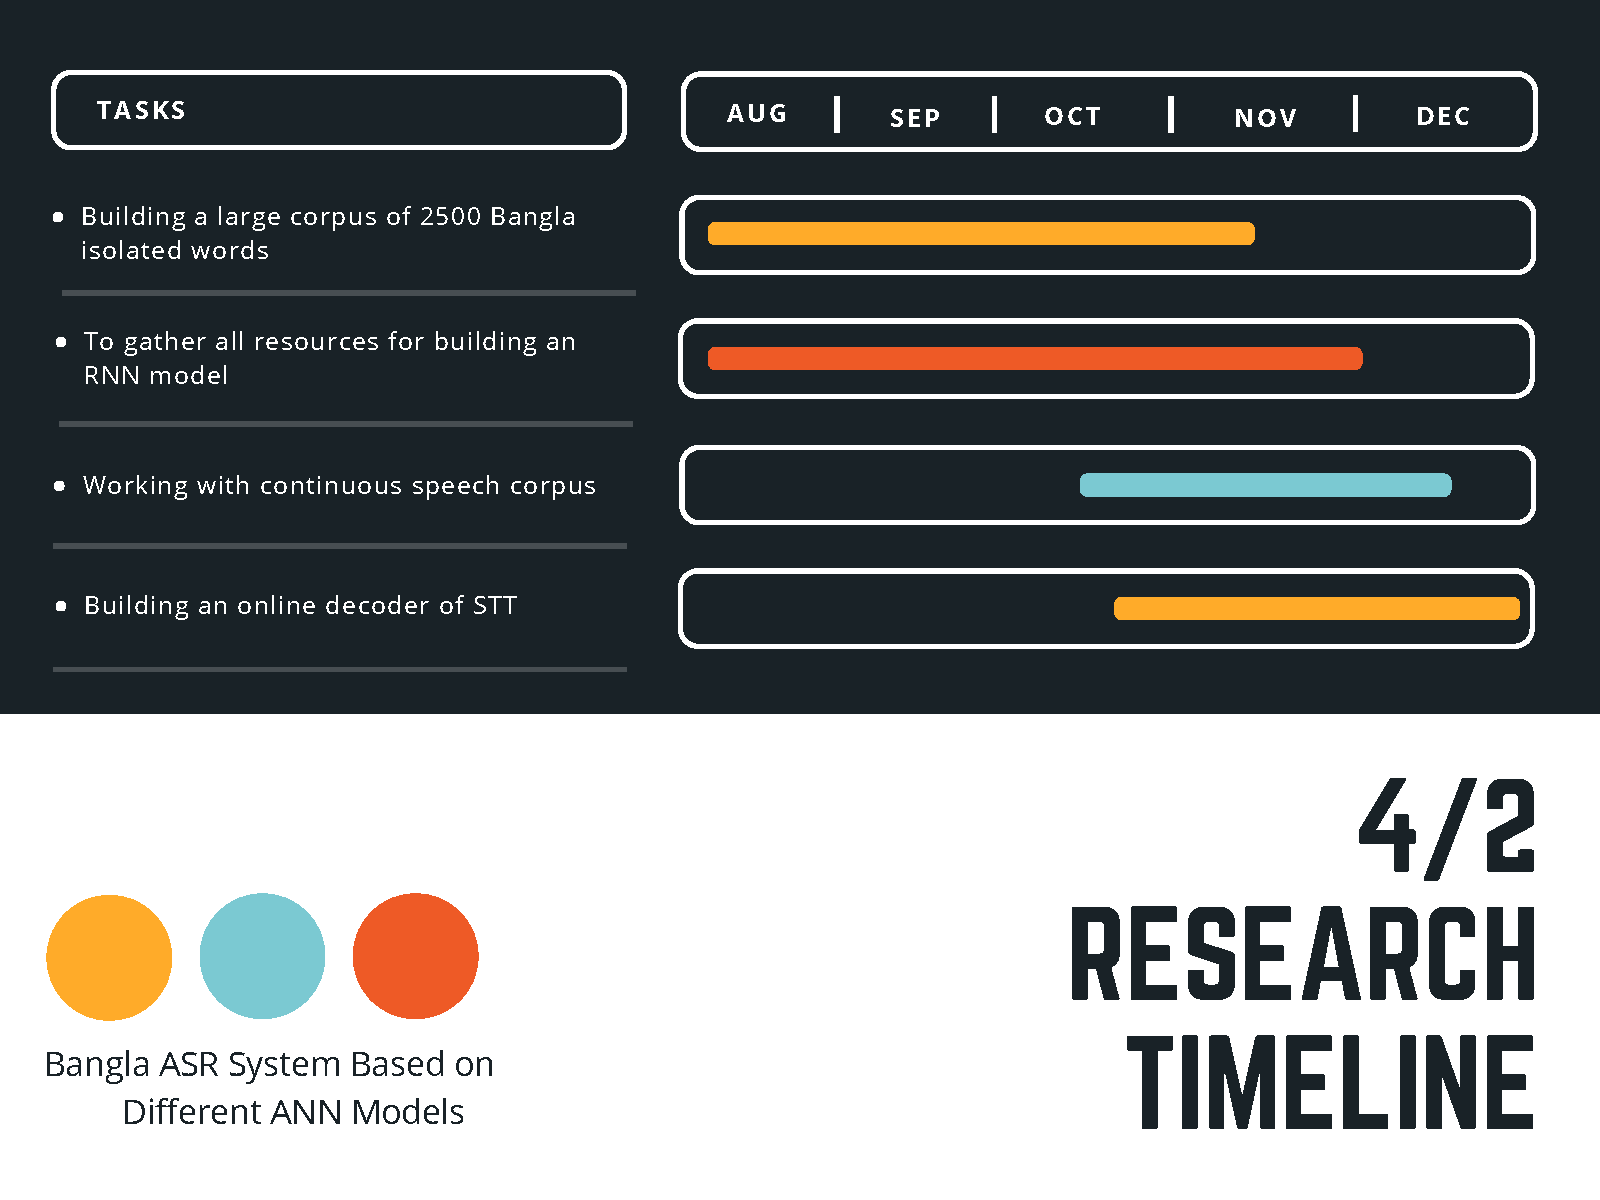
\includegraphics[width=13cm, height=7.0cm]{img/FinalSemesterGanttChart.pdf}}
   \caption{Plan of 4/2 Semester}
  \label{fig:FinalSemesterGanttChart}
\end{figure}

\end{document}